\chapter{Desarrollo de la solución propuesta}
\label{cap:descrip}

Una línea de extrusión completa está compuesta por distintos componentes. En la Figura \ref{fig:esquema_extrusora} vemos los elementos que lo conforman, así mismo, vemos que en cada uno de ellos, hay diferentes valores que influyen en la calidad final del filamento.

\begin{figure}[H]
    \centering
    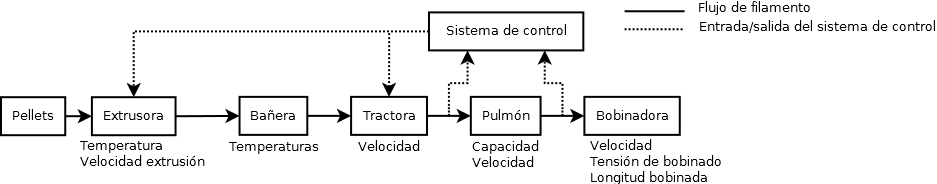
\includegraphics[width=0.99\textwidth]{images/esquema_extrusion.png}
    \caption[Esquema de los elementos que conforman una extrusora.]{Esquema de los elementos que conforman una línea de extrusión completa. Vemos el flujo de avance del filamento según sale de la extrusora y pasa por los distintos elementos. Según el sistema de control se leera el diámetro del filamento antes o después del pulmón, para actuar sobre el motor de la extrusora o de la tractora.}
    \label{fig:esquema_extrusora}
\end{figure}

En una línea de extrusión convencional, se tiene acceso visual a los parámetros indicados, sin embargo no queda registrado en ningún lugar de cuales han sido. Hasta que la extrusión de filamento no se ha extendido, no era necesario tener en detalle estos valores, ya que eran pocos los parámetros que afectaban a la calidad del perfil extruido. Sin embargo, en la extrusión de filamento, son muchos los valores que pueden afectar a la calidad del producto final.\\

Por estos motivos y poder tener una gestión de calidad del producto fabricado, se decide desarrollar un sistema de adquisición de datos para que se pueda hacer una trazabilidad completa de los parámetros de fabricación.\\

\section{Planificación}
\label{sec:planificacion}

El proyecto está definido por dos fases:\\

La primera fase en la que se desarrollará el sistema de adquisición de datos constará de los siguientes puntos:

\begin{itemize}
    \item Recopilación y análisis de la documentación de todos los dispositivos de interés para el proyecto de la línea de extrusión.
    \item Definición de los requisitos respecto a comunicaciones necesarias entre los dispositivos de la línea y el sistema de adquisición.
    \item Determinar los requisitos del autómata progamable industrial (PLC) a utilizar.
    \item Programación del PLC. Puesto que será el encargado de llevar el control de la planta, deberemos programar la adquisición de datos para establecer el control sobre la linea.
\end{itemize}

En esta fase se pondrá en marcha todo el sistema en la planta, instalando el PLC y cableando toda la red de comunicaciones y sensores que disponemos. Así mismo se almacenarán datos de los sensores de temperatura que dispone la planta y el sensor de diámetro. Con los datos adquiridos se modelará parcialmente la planta para intentar hacer un control en lazo cerrado entre la unión tractora de filamento y el sensor de diámetro del mismo. Durante esta fase se diseñará un sistema, para poder visualizar los datos adquiridos de forma remota.\\

De forma general, una linea de extrusión controla el filamento actuando sobre dos velocidades, la de extrusión o la de tracción. La tractora es la encargada de tirar del filamento según salga de la extrusora. Lo habitual es variar la velocidad de la tractora en función del diámetro que se tenga pero también se suele variar la velocidad de extrusión, sin embargo esto puede afectar a la calidad del filamento, puesto que no todo el material estará el mismo tiempo en la extrusora pudiendo generar una degradación en los pellets.\\

Para poder investigar acerca de qué método de control es mejor se realizará un estudio de diferentes sistemas de control para regular el diámetro final del filamento. Se estudiarán los beneficios de usar distintos tipos de controladores como pueden ser PID, control borroso, etc. para posteriormente estudiar los beneficios e inconvenientes de cada uno de ellos.\\

Los plazos asignadaos a cada una de las distintas fases que componen el proyecto, se puede ver en el Anexo \ref{ane:gant}

\section{Herramientas empleadas}
\label{sec:herramientas}

Para el desarrollo de las distintas partes del proyecto, ha sido necesario utilizar varios programas informáticos que nos han ayudado en la consecución de los objetivos del mismo. A continuación, se introducen brevemente, los programas usados más importantes.
\begin{itemize}
\item{GitHub: es una plataforma de desarrollo colaborativo en el que se pueden alojar proyectos utilizando la herramienta de control de versiones Git. El código almacenado en esta plataforma es de dominio público, sin embargo también existe la posibilidad de crear repositorios privados creándonos una cuenta de pago. Para la realización del proyecto se ha creado un repositorio online \cite{githubTFG} en el que se han ido subiendo todos los ficheros que se han ido utilizando para la realización del mismo.}

\item{GNU Octave:  programa libre para realizar cálculos numéricos. Ofrece un interprete de comandos, donde se van escribiendo los comandos que queramos realizar. También permite mostrar gráficas con una serie de datos numércios. Se le considera el equivalente a Matlab \cite{octave}. Esta herramienta se ha utilizado en el proyecto para calcular el modelo matemático de un sistema, para la posterior implementación de un regulador PID.}

\item{Autodesk Inventor: 
Durante la ejecución del proyecto, ha sido necesario realizar piezas específicas a nuestras necesidades. Para ello se han usado impresoras 3D y diseñado las propias piezas que en cada momento han sido necesarias. El diseño de las mismas ha sido realizado en la herramienta Autodesk Inventor. Esta herramienta ofrece un paquete de modelado de sólidos en 3D profesional que compite con otros programas de diseño asistido por ordenador, como pueden ser Catia, Pro/ENGINEER y Solid Edge entre otros.

\begin{figure}[H]
    \centering
    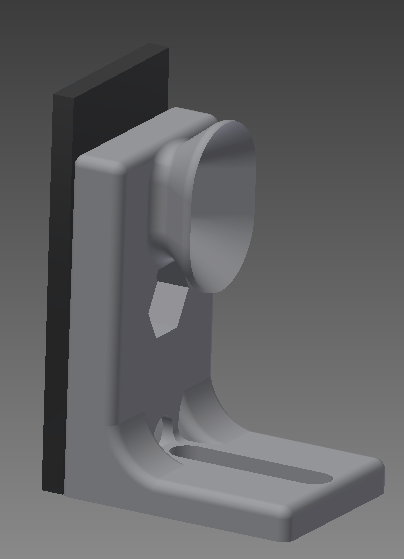
\includegraphics[width=0.25\textwidth]{images/peletizadora/guia.png}
    \caption[Ejemplo de pieza diseñada con Autodesk Inventor.]{Ejemplo de pieza diseñada con Autodesk Inventor. En la Figura vemos una pieza específica diseñada para el proyecto.}
    \label{fig:pieza}
\end{figure}
}
\item{Cura 15.02.1: 
Para la fabricación de las piezas diseñadas, se han usado impresoras Witbox y un software capaz de laminar el fichero STL en G-code para que la impresión de la pieza sea correcta. En este software es donde se conFiguran los parámetros de fabricación final de la pieza.

\begin{figure}[H]
    \centering
    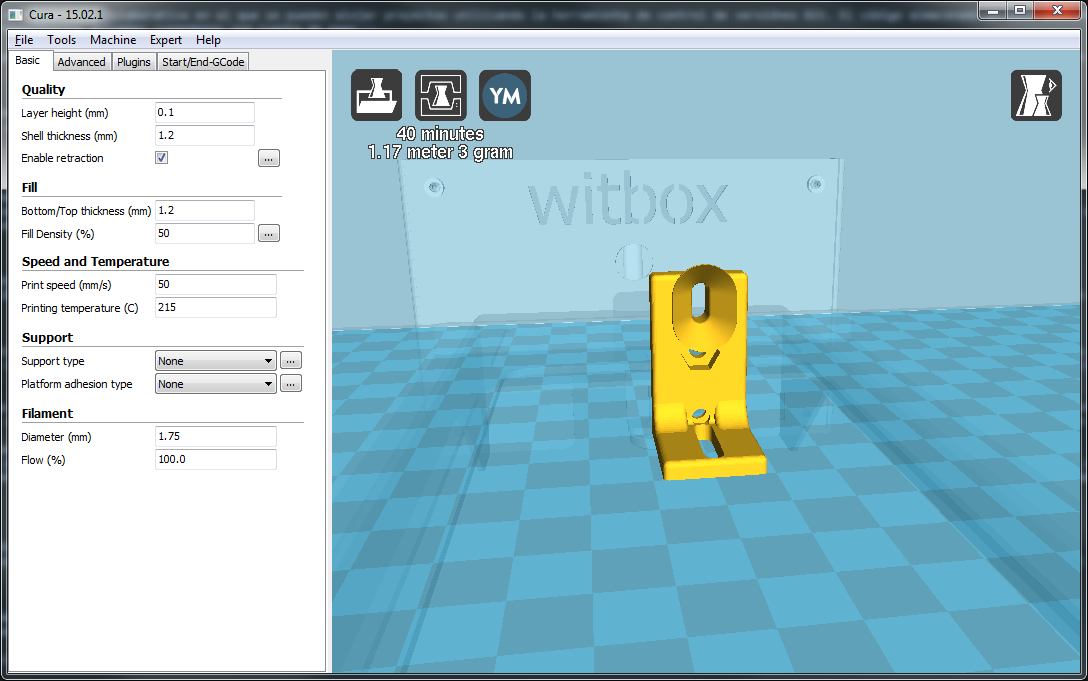
\includegraphics[width=0.7\textwidth]{images/cura.png}
    \caption[Pieza diseñada abierta en cura.]{Pieza diseñada abierta en cura. Podemos ver como en el laminador se pueden conFigurar los distintos parámetros de fabricación de la pieza.}
    \label{fig:cura}
\end{figure}}

\item{
IPython: es una consola de Python mejorada, la cual añade mejoras como puede ser resaltado de líneas, coloreado de sintaxis, autocompletado entre otras ventajas \cite{PER-GRA:2007}. Además ofrece una interfaz tipo notebook lo cual añade la posibilidad de combinar ejecución de código python, mostrar texto matemático, gráficas y contenido múltimedia \cite{ipython}. Estos notebooks son interactivos y permiten observar cómo se han realiado los cálculos y análisis. Podemos ver un ejemplo en la Figura \ref{fig:ipython}.

\begin{figure}[!ht]
    \centering
    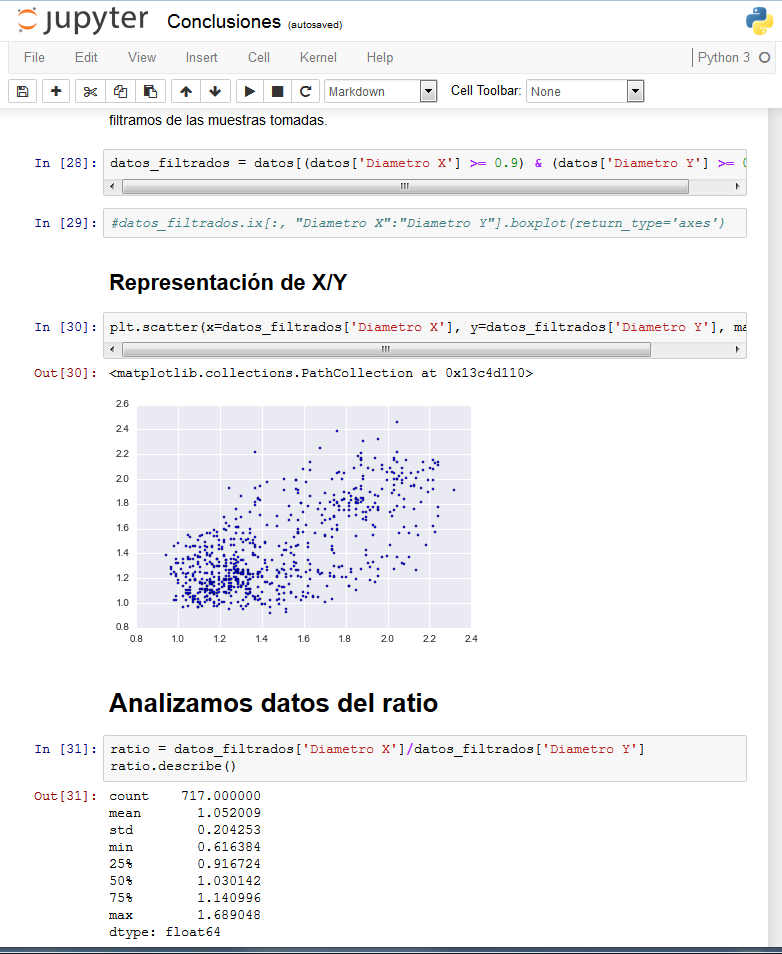
\includegraphics[width=0.5\textwidth]{images/ipython.png}
    \caption[Ejemplo de iPython Notebook usado en el proyecto.]{Ejemplo de iPython Notebook usado en el proyecto. En la Figura vemos, como se puede combinar texto plano, ejecución de código Python y mostrar gráficas.}
    \label{fig:ipython}
\end{figure}

Esta herramienta se ha utilizado en el proyecto para poder calcular el modelo matemático de un sistema e implementar un regulador PID, así mismo, se han analizado los datos adquiridos durante una producción de filamento y comprobar los resultados del sistema diseñado. Los cuadernos realizados están disponibles para su consulta y descarga en el repositorio que se ha creado para el proyecto \cite{githubTFG}.}

\item{Automation Builder ABB: 
Es el entorno de desarrollo para automátas programables de ABB. Desde él se pueden configurar las opciones usadas en el automáta programable así como los módulos de expansión usados. Incorpora CodeSys, un editor de código para desarrollar el programa de control en diferentes lenguajes de programación, además de gestionar las librerias software que necesitemos en el proyecto.\\

Desde este herramienta, podremos incorporar distintos servicios de RED al PLC, como pueden ser un servidor de páginas web (HTTP) y un servidor de transferencia de ficheros (FTP).}
\end{itemize}
\section{Elección de los componentes}

Se quiere desarrollar un sistema capaz de leer información de varios sensores y dado el caso activar elementos de control, todos ellos situados en un entorno industrial como es una fábrica de extrusión de polímeros. Por ello, el sistema elegido debe ser lo más robusto posible y tener capacidades de expansión por módulos para que, según la línea en la que se instale, se pueda acceder a una gran variedad de sensores.\\ 

Así mismo, el sistema debe tener la posibilidad de almacenar información en una memoria externa, ya sea, alojada dentro del mismo sistema o en un sistema externo, como puede ser un servidor de bases de datos. También, debe poder estar conectado a una red ethernet con acceso a Internet, para poder acceder de forma remota desde fuera de la fábrica.\\ 

Debido a todas estas características, se decide usar como unidad central del sistema, un autómata programable industrial (PLC) que en una primera aproximación parece ser lo más adecuado. También se intenta buscar un PLC que nos ofrezca las siguientes ventajas, no siendo estas imprescindibles, pero si ayudarán a la hora de elegir un modelo u otro:

\begin{itemize}
		\item{Licencia de desarrollo libre.}
		\item{Modelo básico con el mayor número de especificaciones necesarias.}
		\item{Capacidad de expansión de las características por medio de módulos.}
\end{itemize}

De este modo, conseguimos reducir el coste total del proyecto. Partiendo de estos requisitos y buscando distintos proveedores por Internet, las empresas que mejor se ajustan son:

\begin{itemize}
		\item{\textbf{UNITRONICS:} La compañía ofrece un PLC con pantalla HMI de bajo coste, que es idóneo para pequeños proyectos que no requieran demasiada capacidad. El principal problema es que no dispone de ninguna expansión para almacenar en tarjetas SD, ni se tiene conocimiento de que se pueda conectar a una base de datos MYSQL de forma directa.}
		\item{\textbf{WAGO:} Cumple todos los requisitos que necesitamos, sin embargo, es necesario pagar una licencia para poder usar el software disponible}
		\item{\textbf{ABB:} El PLC de la gama eco trae de serie la mayoría de las cosas que necesitamos, además, si no se superan ciertas limitaciones, no es necesario pagar una licencia para poder usar el software de desarrollo.}
\end{itemize}

El PLC que se adquiere es de la marca ABB debido a la gran relación calidad precio que ofrece. Una vez adquirido el PLC lo siguiente será realizar el montaje del armario donde irá colocado en la fábrica. En el anexo \ref{ane:plc} se detalla el proceso de construcción que se ha llevado acabo.\\

Para poder demostrar que el sistema a desarrollar es válido para resolver el problema planteado, se mantienen conversaciones con los responsables de PESL para poner en común cuales son los dispositivos que disponen en la fábrica, sin embargo, debido a planificaciones de producción que tienen PESL solo se disponen de dos líneas de extrusión, resulta imposible destinar una línea de fabricación para poner en marcha nuestro sistema.\\

Debido a ello, se decide adquirir una extrusora de laboratorio y poder implementar el sistema en ella desde su instalación por parte del distribuidor. Sin embargo, los plazos de entrega estipulados, se alejan de la fecha de presentación del presente proyecto y por ese motivo se decide usar una extrusora casera que se tiene en el departamento de robótica e innovación de BQ (ver Figura \ref{fig:hardware_filastruder}).

    \begin{figure}[H]
            \centering
            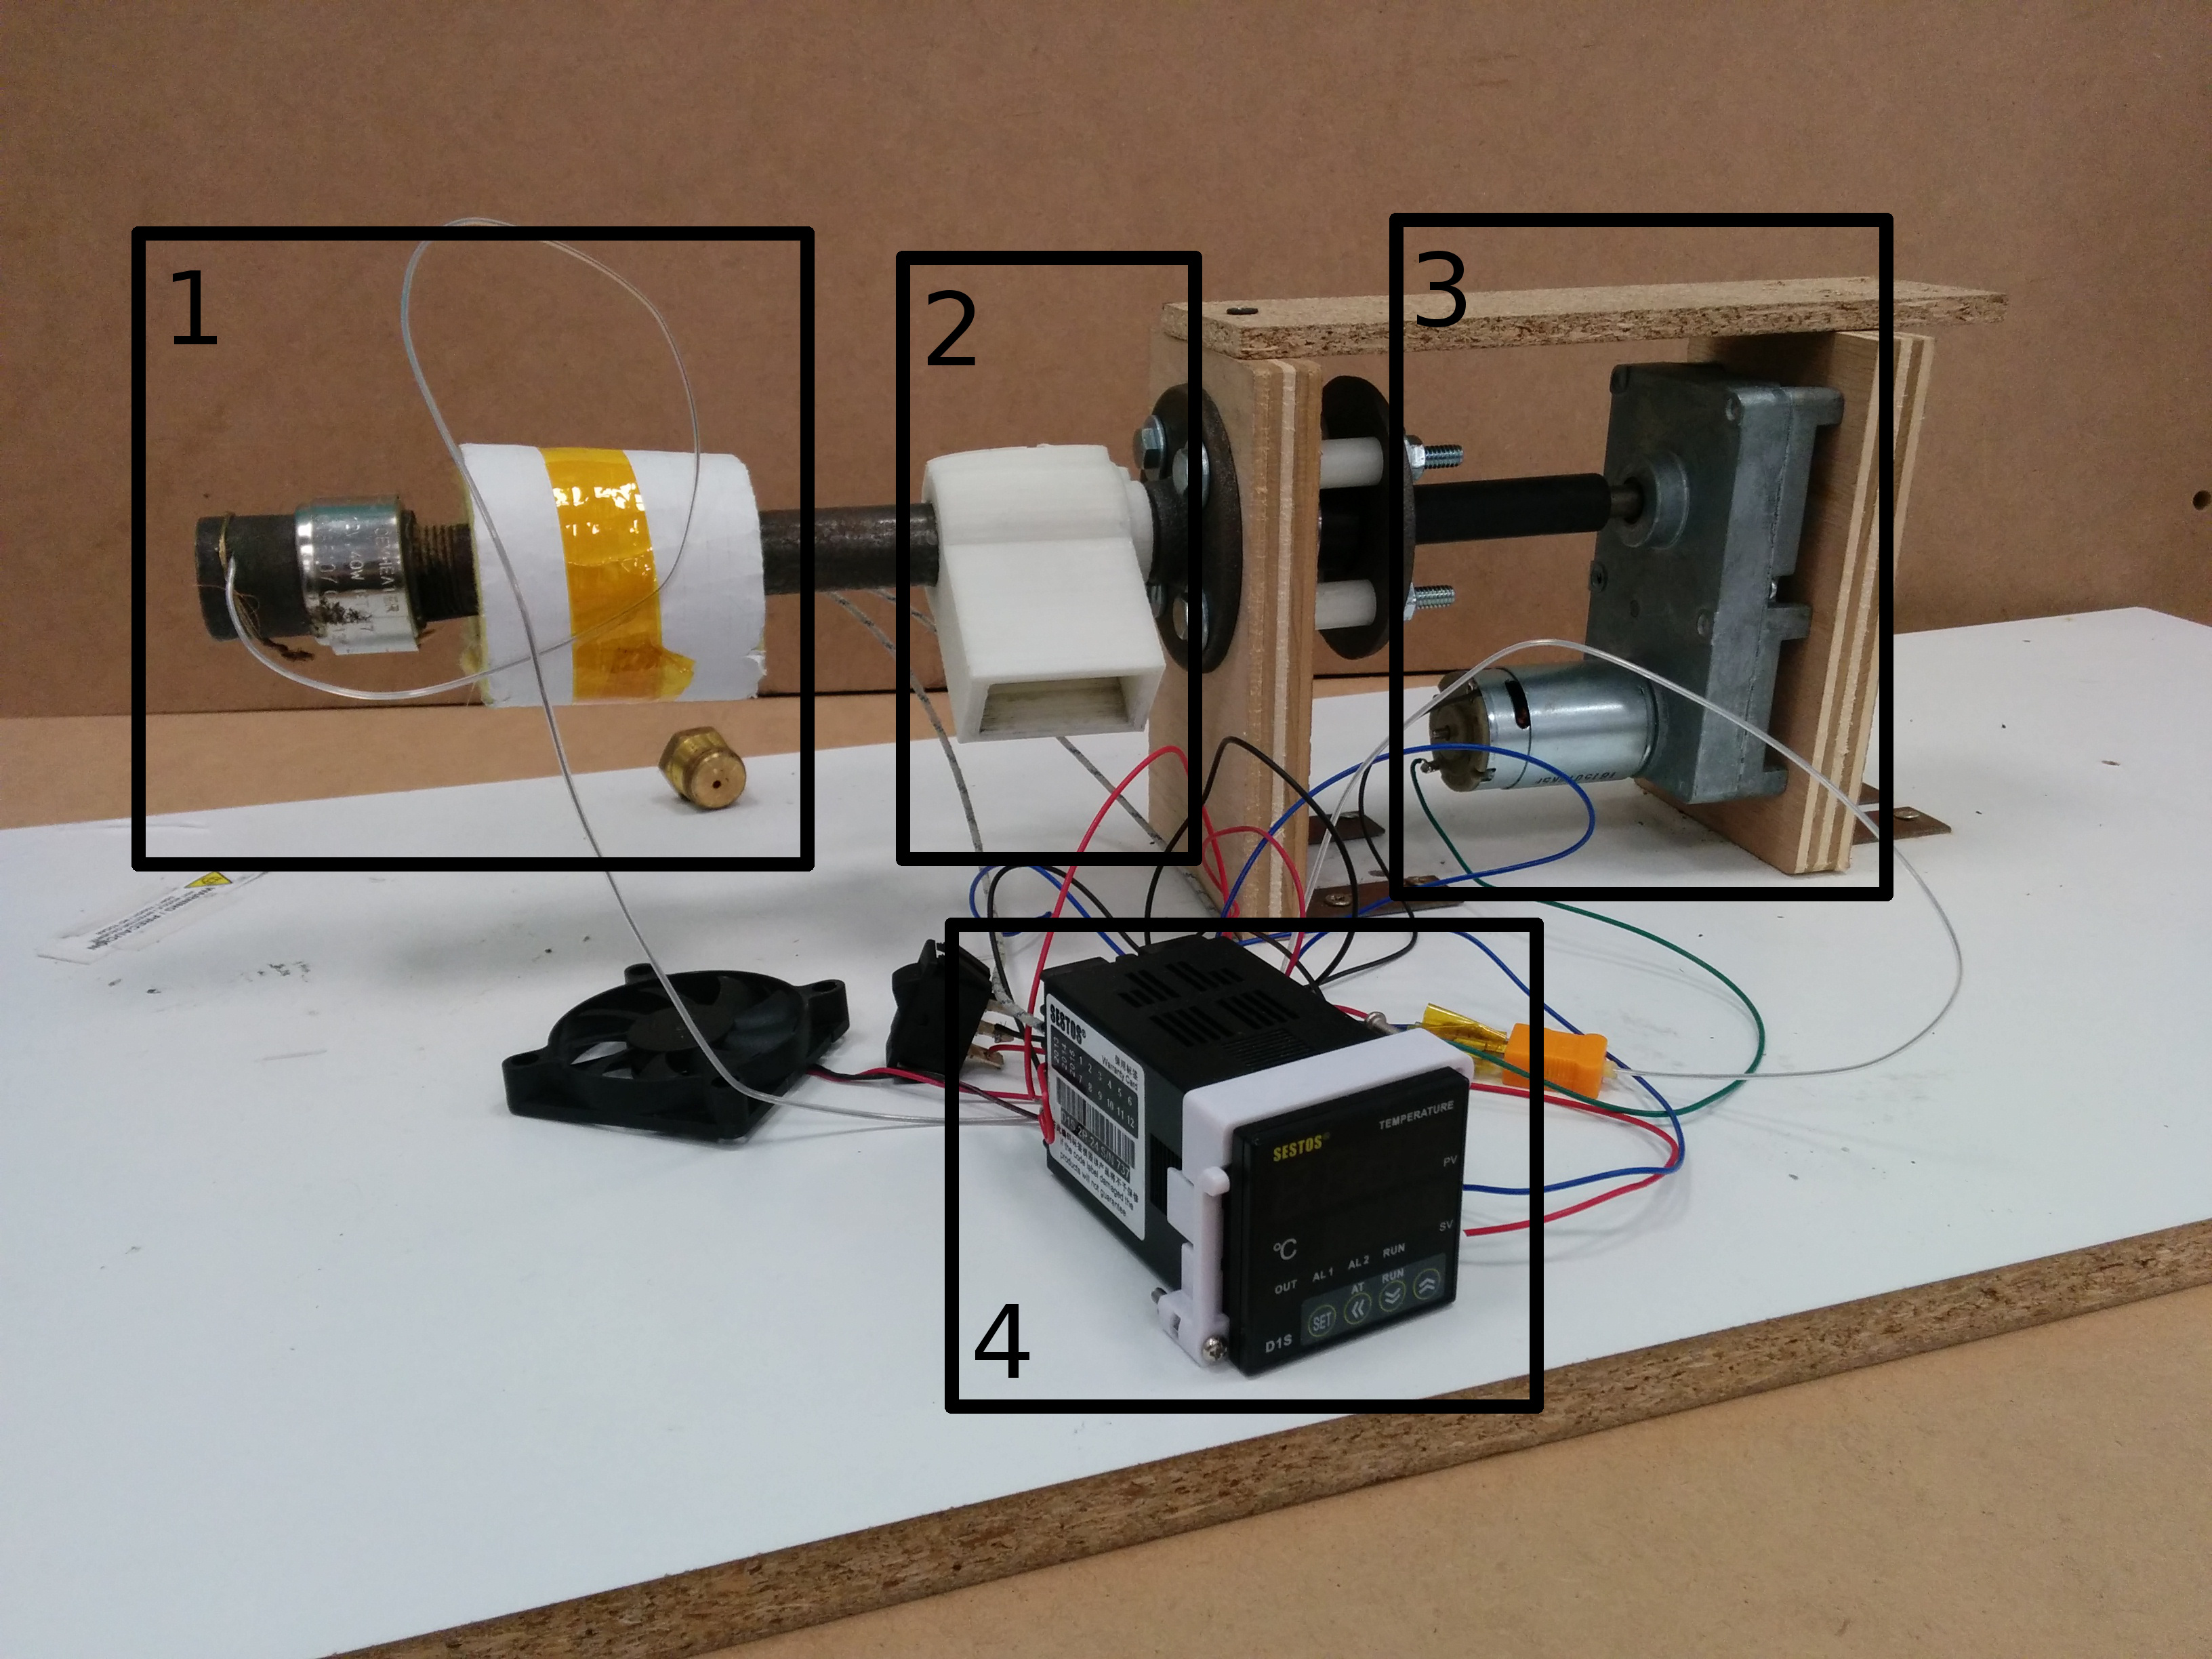
\includegraphics[width=0.6\textwidth]{images/filaextruder/IMG_20150313_11163.jpg}
            \caption[Maqueta de filastruder montada]{Maqueta de filastruder montada. (1) Boquilla y calefactor de la extrusora. (2) Tolva de alimentación de material. (3) Motor para mover el husillo. (4) Controlador de temperatura.}
            \label{fig:hardware_filastruder}
    \end{figure}

Filastruder se presenta como proyecto en Noviembre de 2012 \cite{filastruder} y consiguió recaudar $212.278 \$$ en una campaña de crowfunding en kickstarter\footnote{https://www.kickstarter.com/projects/833191773/filastruder-a-robust-inexpensive-filament-extruder?lang=es}. Es un extrusor de baja capacidad y de bajo coste debido a que el usuario es el que realiza el proceso de montaje, liberado como Open Source (DIY). Todo el proceso de construcción del extrusor se documentó en el foro y se creó una comunidad de usuarios interesados en los extrusores caseros.\\

Algunas de las características de este extrusor son:

\begin{table}[H]
    \centering

        \begin{tabular}{lc}
        \textbf{Par de detenimiento del motor}            & $12N.m$                           \\
        \textbf{Velocidad del motor}                      & $3 rpm$                           \\
        \textbf{Tiempo para extruir 1kg}                  & $24H$                             \\
        \textbf{Diámetro del husillo}                     & $15.875mm$                        \\
        \textbf{Longitud del husillo}                     & $255mm$                           \\
        \textbf{Tolerancia declarada}                     & $\pm 0.05 mm$                     \\   

    \end{tabular}
    \caption[Características filastruder.]{Características filastruder. Fuente\cite{tfg_diego}}
    \label{tab:caract_filas}
\end{table}

Pese a que el funcionamiento no es el adecuado para crear un filamento de calidad, si es completamente útil para la realización del proyecto. Ya que con dos sensores de temperatura, dos cartuchos calefactores y un sensor de diámetro, podremos simular una extrusora industrial, de esta manera también, demostramos que el sistema es totalmente escalable y con cambios en el software podremos adquirir datos de cualquier extrusora. En el Anexo \ref{ane:filastruder} se detalla el proceso llevado a cabo para montar la filastruder.\\

Se decide usar un sensor de diámetro opensource del cual, toda la información necesaria para su construcción está accesible via online \cite{thing_filamento}. En el Anexo \ref{ane:sensor} se detalla el proceso llevado a cabo para su construcción.\\

A la hora de obtener matería prima para poder extruir filamento, se decide construir una peletizadora (ver Anexo \ref{ane:peletizadora}), maquina capaz de reciclar filamento que no cumple las condiciones para ser usado en una impresora 3D, de esta manera, podríamos abaratar costes, evitando tener que usar pellets de PLA para un filamento que no sabemos si va a ser utilizable. Antes de extruir el filamento, se comprueba si los pellets reciclados son aptos para la extrusión.\\

Por ello, se realizan ensayos por calorimetría diferencial de barrido (DSC). El DSC es una técnica que permite el estudio de las transiciones de fase en los materiales polímeros \cite{DSC1} lo que es de suma importancia a la hora de establecer sus condiciones de procesado y aplicaciones tecnológicas, ya que el tipo de fases y transiciones entre ellas determinan su comportamiento físico macroscópico.\\

Estos ensayos son realizados por Javier Arranz Andrés, compañero del departamento. Las medidas se hicieron en un calorímetro TA Instruments Q20 con sistema de enfriamiento y bajo atmósfera de nitrógeno. El aparato se calibró con Indio como sustancia de referencia ($Tm = 156.6 ^o C$, $\delta H = 28.45 J/g$). En el ensayo se sometió al polímero a una fusión a $20 ^o C/min$, seguida de una cristalización y una segunda fusión, a la velocidad de $5 ^o C/min$.\\

Se empleó el calor de fusión del PLA $100\%$ cristalino, 93 J/g \cite{DSC}. Los errores en la determinación de las temperaturas, en el cálculo de la entalpía y en el de la cristalinidad se estimaron en $\delta1 ^o C$, $\pm4 J/g$ y $\pm0.04$ respectivamente. El peso de las muestras osciló entre 6 y10 mg, y las temperaturas de transición, Tm y Tc se tomaron en el punto máximo de la curva endoterma o exoterma. La Tg se tomó a la temperatura en la que se alcanza la mitad de la diferencia de calor específico existente entre el estado amorfo vítreo y el amorfo elastómero, es decir $T_{g} = 0.5 \pm C_{p}$.\\

A continuación se incluyen los resultados obtenidos en el experimento. En la Figura \ref{fig:analisis_dsc} se observa cómo en condiciones térmicas de temperatura de transición vítrea (Tg) y temperatura de fusión, ambos filamentos son prácticamente iguales. Como vemos en la tabla \ref{tab:dsc2} no ocurre lo mismo con el grado de cristalinidad del polímero, el cual difiere de uno a otro, sin embargo la diferencia está dentro del margen de error experimental. Esta diferencia puede ser un indicador de inicio de degradación, debido a que las cadenas del polímero son más pequeñas y dificultan el movimiento en sus partes extremas dificultando la cristalinidad. A falta de realizar un ensayo de propiedades mecánicas de ambos filamentos y con el ensayo realizado, podemos dar como válido el pellet reciclado con la peletizadora para su uso en la extrusión del mismo.

\begin{figure}[H]
    \centering
    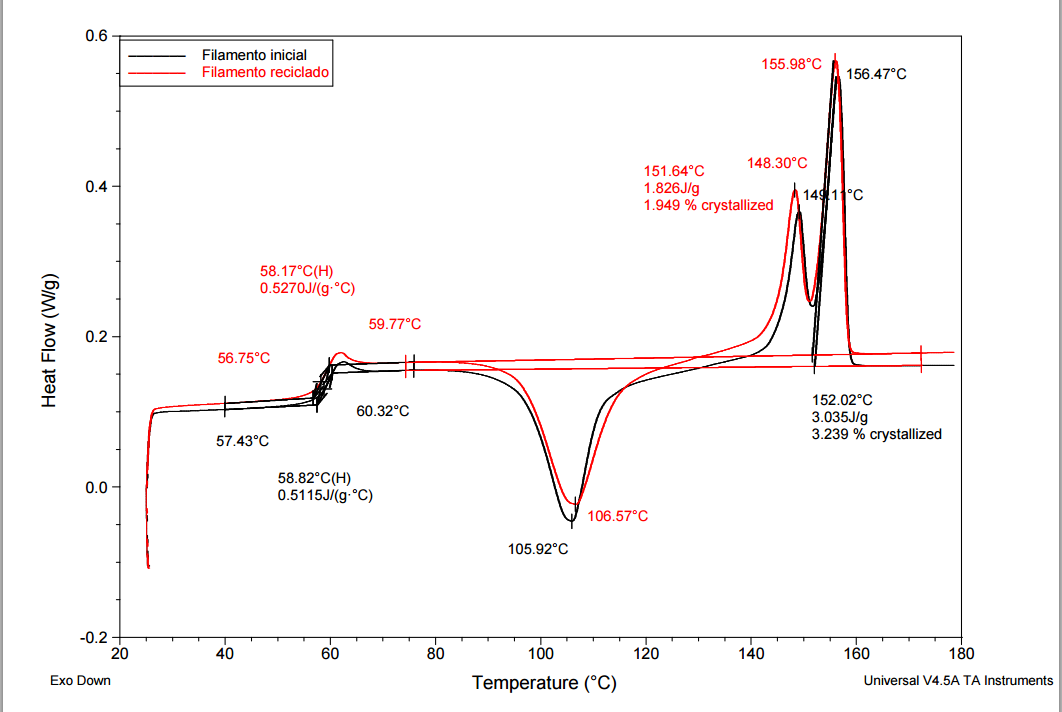
\includegraphics[width=0.9\textwidth]{images/dsc2.png}
    \caption[Resultado del análisis con DSC de filamento reciclado.]{Resultado del análisis con DSC de filamento reciclado. Vemos el filamento original (color negro) comparado con el filamento reciclado (color rojo). Podemos llegar a la conclusión de que el filamento reciclado es apto para reutilizar.}
    \label{fig:analisis_dsc}
\end{figure}

En las Tablas \ref{tab:dsc1} y \ref{tab:dsc2} podemos ver los datos obtenidos:

\begin{table}[H]
    \centering
    \begin{tabular}{llllll}
        \multicolumn{6}{c}{Glass Transition}                                                        \\
                            & Onset (ºC) & Midpoint (ºC) & End (ºC) & Height W/g & Delta Cp (J/gºC) \\ \hline
        FIlamento Inicial   & 61.0      & 56.0         & 50.5    & 0.04    & 0.5           \\
        Filamento reciclado & 60.5     & 55.5         & 50.5    & 0.04    & 0.5         
    \end{tabular}
    \caption[Datos del DSC con la transición vítrea del filamento.]{Datos del DSC con la transición vítrea del filamento. En los resultados podemos observar, cómo apenas se produce una degradación en las propiedades térmicas del material reciclado, siendo los valores, muy similares de una muestra a otra}
    \label{tab:dsc1}
\end{table} 

\begin{table}[H]
    \centering
    \begin{tabular}{lllll}
        \multicolumn{5}{c}{Peak Integration}                                                                                 \\
                             & Midpoint (ºC) & Stop (ºC) & Area J/g   &  \% crystalized \\ \hline
        Filamento Inicial    & 93.0         & 70.0     & 2   &  3                         \\
        Filamento reciclado  & 91.0        & 70.0     & 1    & 2                        
    \end{tabular}
    \caption[Datos del DSC con la cristanilidad del filamento]{El único dato que difiere de un filamento a otro, es el porcentaje de cristanilidad, sin embargo la diferencia entre ambas medidas está dentro del error experimental.}
    \label{tab:dsc2}
\end{table}


\section{Programación del PLC.}

Disponemos de todo el material necesario para la realización de una pequeña extrusora de filamento y la adquisición de sus datos más característicos en la producción. El siguiente paso es desarrollar la programación del PLC para realizar las tareas de control y adquisición de datos.

Los requisitos que debe tener el sistema se enumeran a continuación y se detallan en las secciones posteriores:

\begin{itemize}
    \item{Controlar la temperatura del extrusor.}
    \item{Controlar motor del husillo.}
    \item{Leer información del sensor de diámetro.}
    \item{Almacenar la información tomada en un fichero de datos.}
    \item{Visualizar en una página web el estado de la producción.}
\end{itemize}

Para desarrollar el software que gestione el PLC, se usa una máquina de estados en la que pasando por diversos estados, se irán ejecutando las acciones de control. Debemos entrar en modo producción mediante la activación de una variable. Si estamos en producción, pasaremos por los distintos estados y mientras no estemos en producción, las salidas digitales y valores de consigna de los PID son reseteados a cero como medida de seguridad. Una vez que entremos en producción, el primer paso es inicializar el programa, generamos el nombre del fichero donde almacenamos los datos. Después se genera el fichero CSV y en caso de que no se produzca ningún error, se almacena la cabecera en el fichero CSV, para pasar a la producción como tal. Se controlará la temperatura del dado, se registrarán los valores de diámetros y temperaturas y se irán almacenando en el fichero CSV.\\

La máquina de estados se muestra en la Figura \ref{fig:plc_estados}

\begin{figure}[H]
    \centering
    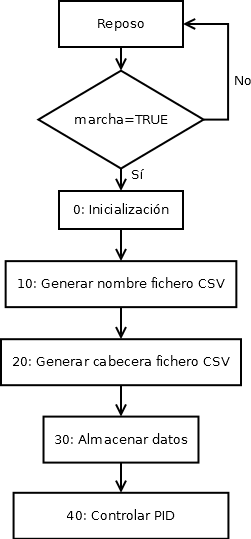
\includegraphics[width=0.25\textwidth]{images/PLC/diagrama.png}
    \caption[Diagrama de estados PLC.]{Diagrama de estados PLC.}
    \label{fig:plc_estados}
\end{figure}

\subsection{Control de la temperatura del extrusor}
\label{sec:plc_PID}

Se implementa un regulador PID para regular la temperatura del extrusor. Es necesario conocer la planta del sistema que queremos regular para implementar de forma correcta el PID. En nuestro caso el sistema a controlar es el calentamiento del dado, por ello, debemos modelar primeramente el sistema. En la Figura \ref{fig:plc_sistema} podemos ver un esquema de un sistema con un regulador PID:

\begin{figure}[H]
    \centering
    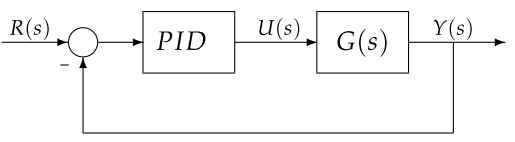
\includegraphics[width=0.4\textwidth]{images/PLC/sistema.png}
    \caption[Sistema con un regulador PID.]{Sistema con un regulador PID. La salida del sistema tendrá una realimentación a la entrada del regulador, para tomar acción de control.}
    \label{fig:plc_sistema}
\end{figure}

Con ayuda del programa que se desarrolla en el PLC haremos las siguientes tareas:

\begin{itemize}
    \item{Almacenar los datos de la temperatura en el dado.}
    \item{Encender de forma controlada la resistencia de calentamiento.}
\end{itemize}

Una vez realizadas, analizaremos los datos guardados, para ver como se comporta el sistema en lazo abierto, sin ningún tipo de control. Partiendo de una temperatura ambiente, se registran los valores de las temperaturas para a continuación encender la resistencia de calentamiento y ver cómo la temperatura va aumentando a medida que pasa el tiempo. Una vez que la temperatura sobrepase un valor que nosotros establezcamos, pararemos el experimento.\\

Mediante un script programado con Python y varias herramientas de análisis de datos como: IPython, Scipy, Pandas y Numpy, analizamos los datos obtenidos, para ver cómo se comporta nuestro sistema. Las graficas en la Figura \ref{fig:plc_lazo_abierto} muestra la respuesta en el tiempo de nuestro sistema de calentamiento, sin ningún tipo de control.

\begin{figure}[H]
    \centering
    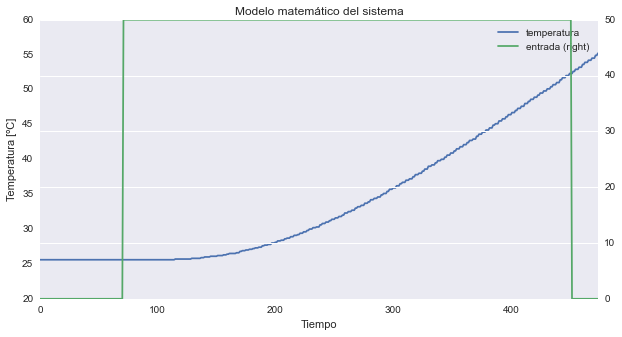
\includegraphics[width=0.99\textwidth]{images/PLC/modelado/modelado_9_1.png}
    \caption[Respuesta del sistema en lazo abierto]{Respuesta del sistema en lazo abierto. Observamos como a medida que avanza el tiempo, también lo hace la temperatura de manera exponencial.}
    \label{fig:plc_lazo_abierto}
\end{figure}

Para poder controlar de forma óptima el sistema, es necesario calcular la ecuación matemática que mejor se ajuste a nuestros datos y con ella el polinomio que caracteriza nuestro sistema. Ña Figura \ref{fig:plc_lazo_abierto2} muestra una curva ajustada

\begin{figure}[H]
    \centering
    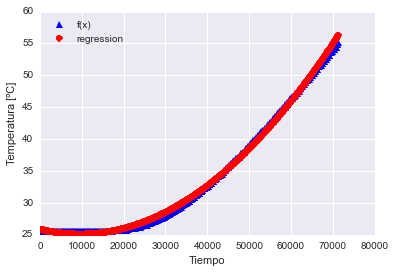
\includegraphics[width=0.8\textwidth]{images/PLC/modelado/modelado_13_1.png}
    \caption[Ajuste de la recta.]{Ajuste de la recta. Calculamos el polinomio que mejor se adapte a nuestros datos.}
    \label{fig:plc_lazo_abierto2}
\end{figure}

\begin{equation}
P_x=  25.9459 -1.5733 \cdot 10^{-4} \cdot X - 8.18174 \cdot 10^{-9} \cdot X^2
\end{equation}

\noindent{Si calculamos la transformada de Laplace del sistema, obtenemos la planta de nuestro sistema, con la cual podremos implementar el regulador PID:}

\begin{equation}
G_s = \frac{25.95 \cdot S^2 - 0.00015733 \cdot S + 1.63635 \cdot 10^{-8}}{S^3}
\end{equation}

\noindent {Aplicando el método de sintonizacion de Ziegler-Nichols \cite{zn} basado en la curva de respuesta, calcularemos el PID para poder regular correctamente el sistema. Este método consiste en estudiar el sistema en lazo abierto con escalón unitario, calculamos parámetros como la máxima pendiente de la curva y el retardo, y establecemos con ellos las ganancias del controlador PID \cite{PID}. Este método no facilita de manera rápida unos valores de $K_p$, $K_i$ y $K_d$ orientativos, para que podamos ajustar correctamente el controlador.} \\

La Figura \ref{fig:plc_PID4} muestra la respuesta al sistema una vez que se ha implementado un regulador PID para controlar la temperatura.

\begin{figure}[H]
    \centering
    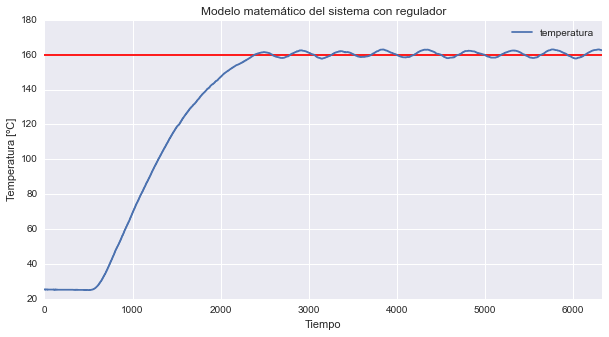
\includegraphics[width=0.99\textwidth]{images/PLC/modelado/modelado_38_1.png}
    \caption[Respuesta del sistema con PID.]{Respuesta del sistema con PID. En la gráfica se aprecia como la temperatura oscila sobre un valor.}
    \label{fig:plc_PID4}
\end{figure}

La sobreoscilación que presenta el sistema la calculamos mediante:

\begin{equation}
M_{p}=\frac{T_{max}-Setpoint}{Setpoint} \cdot 100 = \frac{163-160}{160} \cdot 100 = 1.88\%
\end{equation}

Por lo tanto, el regulador que cumple con las especificaciones deseadas tiene la siguiente ecuación característica:
\begin{equation}
G_s = \frac{150 \cdot S^2 + 6082.6 \cdot S + 121.64}{S}
\end{equation}


\subsection{Lectura de datos del sensor de diámetro}
\label{sec:plc_diametro}

Los sensores de diámetro están conectados a dos entradas analógicas de tensión del PLC. Será necesario unir la señal de masa (GND) del PLC con la del sensor, para que la referencia al nivel de tensión $0 V$ sea la misma, posteriormente, la salida del sensor de diámetro, se conectará con la entrada analógica del PLC.\\

El PLC convierte el valor de tensión comprendido entre un rango de 0-10V a un valor numérico, a través de un conversor analógico a digital (ADC) de 10bits, es decir, tenemos una resolución de:

\begin{equation}
    \text{Resolución}=\frac{ V_{max} } {2^{10} } = \frac{10}{1024} = 9.76 mV
\end{equation}

En la Tabla \ref{tab:reso_adc}, se observan los valores que asigna el ADC:

\begin{table}[H]
    \centering
    \begin{tabular}{|c|c|c|}
        \hline
        {\bf Intervalo}                   & {\bf 0 ... 10V}                                                   & \multicolumn{1}{l|}{{\bf Valor digital}}                       \\ \hline
        Desbordamiento                    & \textgreater 11.7589                                              & 32767                                                         \\ \hline
        Valor de medición desmasiado alto & \begin{tabular}[c]{@{}c@{}}11.7589\\ .\\ .\\ 10.0004\end{tabular} & \begin{tabular}[c]{@{}c@{}}32511\\ .\\ .\\ 27649\end{tabular} \\ \hline
        Intervalo normal                  & \begin{tabular}[c]{@{}c@{}}10.000\\ .\\ .\\ 0.0004\end{tabular}   & \begin{tabular}[c]{@{}c@{}}27648\\ .\\ .\\ 1\end{tabular}     \\ \hline
    \end{tabular}
    \caption[Valores de conversión del ADC.]{Valores de conversión del conversor analógico a digital. Para un valor de tensión dado, se le asigna un valor decimal.}
    \label{tab:reso_adc}
\end{table}

Se va a trabajar con el rango de intervalo normal. Para poder saber el diámetro que está midiendo el sensor, se debe leer la entrada analógica y convertir el valor décimal a un valor de tensión, es decir, convertir el valor digital a analogico (DAC), para ello, con los valores del intervalo normal se calcula la ecuación de la recta que lo caracteriza que en este caso es (ver Figura \ref{fig:plc_DAC})

\begin{equation}
Y = 3.6168 \cdot 10^{-4} \cdot X
\label{ec:recta_ADC}
\end{equation}

\begin{figure}[H]
    \centering
    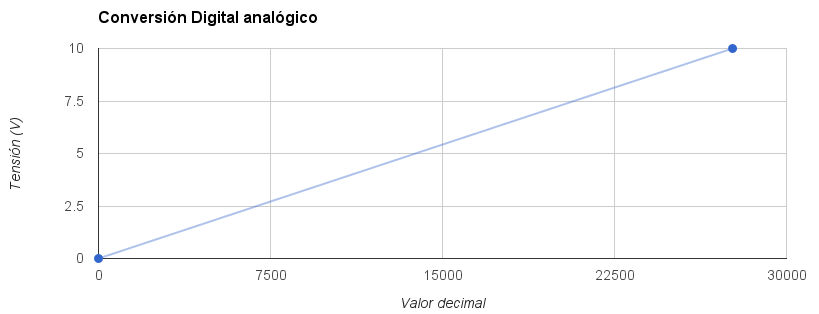
\includegraphics[width=0.75\textwidth]{images/PLC/image.png}
    \caption[Recta característica del ADC.]{Recta característica del ADC. Con su ecuación característica, podemos convertir el valor de tensión a un valor de diámetro.} 
    \label{fig:plc_DAC}
\end{figure}

Con la Ecuación \ref{ec:recta_ADC}, se puede tener acceso al valor del diámetro que tiene el filamento. El siguiente paso entonces, será realizar el almacenamiento de los datos de la producción en un fichero para su posterior análisis.

\subsection{Almacenamiento de la información registrada en un medio físico}
\label{sec:plc_SD}

Se elije un nombre de fichero en el que se usa año, mes, día y minuto para identificar la producción, es decir, tiene un formato \textit{YYMMDDmm.CSV}. El formato elegido para almacenar la información es el de valores separados por coma (CSV). El motivo por el cual se elije este formato es debido a su estandarización y que almacena los datos de forma tabular en texto plano. Gracias a esto, se puede abrir el fichero CSV con cualquier editor de texto y otros programas de hojas de cálculo, para el posterior análisis de los datos, que es uno de los objetivos del proyecto. Por lo tanto, el formato CSV es el idóneo para poder trabajar en el futuro con los datos almacenados.\\

En el progama del PLC se genera una cabecera del fichero CSV, que es la primera fila del fichero, en donde indicará la información que contiene cada columna. La información almacenada en el fichero CSV es la siguiente:

\begin{itemize}
    \item{\textbf{Time Stamp: }Es una secuencia de caracteres en las que se indican hora y fecha de un evento ocurrido. Se almacena con el formato YY-MM-DD HH:MM:SS. Con esta información podremos tener una trazabilidad del filamento almacenado y en caso de producirse un error, ver el momento concreto del mismo.}
    \item{\textbf{Temperaturas: }Valores con las temperaturas del dado y el husillo en la zona de alimentación. De esta manera se comprueba que la temperatura no sufre algún cambio drástico durante el proceso, que puede ser causante de un problema en la calidad final del filamento.}
    \item{\textbf{Diámetros: }Se almacenan los diámetros medidos por el sensor. En este caso se van a poner dos sensores de diámetro para hacer una medición en los dos ejes del filamento.}
    \item{\textbf{Información varia: }Se puede almacenar cualquier información que nosotros deseemos en un futuro (X e Y).}
\end{itemize}

En la tabla \ref{tab:plc_csv} se ve un ejemplo de los datos almacenados en un fichero csv:

\begin{table}[H]
    \centering
    \begin{tabular}{ccccc}
        {\bf Tiempo}         & {\bf Tmp Husillo} & {\bf Tmp Nozzle} & {\bf Diámetro X} & {\bf Diámetro Y} \\ \hline
        2015-8-13 11:11:01  & 67.5              & 150.4            & 1.71         & 1.49         \\
        2015-8-13 11:11:02  & 67.5              & 150.4            & 1.82         & 1.51         \\
        2015-8-13 11:11:04  & 67.5              & 150.5            & 1.91         & 1.52         \\
        2015-8-13 11:11:05  & 67.4              & 150.5            & 1.94         & 1.55         \\
        2015-8-13 11:11:07  & 67.4              & 150.5            & 1.91         & 1.56         \\
        2015-8-13 11:11:09  & 67.4              & 150.6            & 1.92         & 1.58         \\
        2015-8-13 11:11:10 & 67.4              & 150.6             & 1.97          & 1.71         \\
        2015-8-13 11:11:12 & 67.4              & 150.6             & 2.02          & 1.89        \\
                -          &    -              & -                & -                & -
    \end{tabular}
    \caption[Muestra de un fichero CSV con datos de producción.]{Muestra de un fichero CSV con datos de producción. Están registrados los datos más importantes de la producción como son. Time Stamp, Temperaturas y Diámetros.}
    \label{tab:plc_csv}
\end{table}

\subsection{Acceso remoto a los datos de producción}
\label{sec:plc_scada}

La información se almacena en la tarjeta SD interna del PLC a la cual se puede acceder se usa un servidor de transferencia de ficheros (servidor FTP), de esta manera se accede a la SD de forma remota, sin tener que extraer la tarjeta del PLC. En el ordenador, con ayuda de un software cliente FTP se accede a la IP del PLC que se encuentra en la misma red y se descarga el fichero CSV para su posterior estudio.\\

La producción se puede visualizar de forma remota empleando un servidor de páginas WEB en la que se puede acceder al estado de variables del programa y se pueden añadir gráficos que simulen físicamente la planta. Desde esta visualización web se puede:

\begin{itemize}
    \item {Visualización en tiempo real temperaturas de Husillo y Dado.}
    \item {Iniciar y parar producción.}
    \item {Controlar marcha del motor del husillo.}
    \item {Visualizar la ruta del fichero en el que se almacenará la información.}
\end{itemize}

